\documentclass{article}

\usepackage{fullpage}
\usepackage{parskip}
\usepackage{hyperref}
\usepackage{setspace}
\usepackage{mathtools}
\usepackage{tikz}
\usetikzlibrary{arrows}
\usetikzlibrary{decorations.markings}
\usetikzlibrary{calc}
\usepackage{standalone}
\usepackage{float}
\usepackage{caption}
\usepackage{subcaption}
\usepackage{amsmath}
\usepackage{amsfonts}
\usepackage{amsthm}
\usepackage[ruled]{algorithm2e}

\newtheorem{definition}{Definition}
\newtheorem{theorem}{Theorem}
\newtheorem{lemma}{Lemma}

\title{End of Year Progress Monitoring Report}
\author{Geraint Palmer\\{\small Supervisors: Professor Paul Harper \& Dr. Vincent Knight}}
\date{\today}

\begin{document}
\onehalfspacing

\maketitle




\section{Project Overview \& Plan}

This project is supervised by Professor Paul Harper and Dr Vincent Knight. % No need for this
The research will investigate the workforce needs required to care for the frail and the elderly within the Aneurin Bevan University Health Board (ABUHB).
A systems-wide view will be considered to account for the complexity and connectedness of the healthcare system.
Stochastic aspects will need to be captured, such as the variability in patient pathways and resource consumption.

The whole system will be modelled as a queueing network, with nodes representing departments in order to capture general patient flows.
The model parameters will be obtained by exploring and analysing data acquired from the SAIL data bank.
An agent-based simulation model will be created from this model, populated with
the obtained data, where further exploration can be undertaken.

Frail and elderly patients are currently a particular priority for many healthcare planners and managers.
An aging population means an increasing amount of elderly people are accessing healthcare service.
Frail patients tend to have prolonged hospital length of stay partly due to insufficient care at home or in the community.
Patients who remain in hospitals when they could otherwise have returned home block beds, increasing congestion and pressure on other areas of the healthcare system.
This becomes a strain on the workforce, both in hospitals and community care teams.
An understanding of the situation could alleviate this pressure.

% Perhaps here include a pointer for the next subsection? (Always nice to have a
% sentence)

\resultssubsection{Patient Flows}

Queueing theory, and in particular queueing networks are techniques used to model the stochastic flow of customers around a system of service nodes.
Note that throughout this report the terms node, service centre, service node and service station will be used interchangeably.

These concepts have been successfully adapted to healthcare systems, both in detailed individual level systems, e.g. \cite{albinetal90}, \cite{creemerslambrecht07} and in examples with coarser granularity, for example \cite{koizumietal05}.

An example of the sort of queueing network and patient flows that will be modelled is shown in Figure~\ref{fig:healthsystem}.

\begin{figure}[H]
    \includestandalone[width=\textwidth]{images/healthsystem}
    \caption{Patient flows around a healthcare system.}
    \label{fig:healthsystem}
\end{figure}

From exploring data and discussing with professionals at the ABUHB, the general architecture of the health system can be constructed, and patient flows built up.
This will then be modelled as an open queueing network.
Using results from the theory of Jackson networks \cite{You need a reference
here}, performance measures and steady-state probabilities can be obtained.
This model will then be extended to include blocking between nodes so that the model represents reality, in which patients may be unable to progress to their next destination due to lack of capacity.
Again performance measures and steady-state probabilities will be obtained.

A simulation framework has been written in Python \cite{http://www.python.org/},
analytic results will be compared to results obtained through simulation.
A user friendly Django application of this simulation will be built which will
feature simple parameter inputs and graphical outputs.

% add pointer

\subsection{Optimal Routing of Patients}

One interesting avenue to explore is the optimal routing of patients through the system.
That is, when there is a choice of where to send a patient, what is the optimal action to take?
This question will be investigated using reinforcement learning algorithms.

Optimal analytical approaches will be investigated as well as agent based
models. One particular implementation that will be used is
\textbf{reinforcement learning}.

Reinforcement learning is a machine learning technique in which an agent learns
through exploration of their environment, by completing actions and subsequently receiving rewards or punishments.
Overviews are given in \cite{suttonbarto98} and \cite{szepesvari10}.
The \(q\)-learning algorithm will be used to find the optimal action to take given a specific state.

In order to implement this for the queueing network simulation model, the nodes
or service centres will become the agents, the state will be the number of
patients at that node, and the reward will be some function of expected wait. % Put this list in a bullet point list
It will be interesting to see the effect of social vs selfish rewards (that is,
does the node receive rewards according to the system's state or just its own
state), and the difference between nodes observing the whole system's state and
only observing its own state. % This is not a well written sentence.

An extension of the above problem could be finding the optimal routing of
patients when the agents are blind to their state, that is when they are not
aware of the system state.
Some results from game theory, and techniques such as genetic algorithms and
linear programming will be explored.

% Include a pointer.

\subsection{Workforce Planning}

The performance measures from each of the scenarios explored will be used to
compare the workforce needs and skill mix required to care for frail and elderly
patients across the ABUHB. % You have made no mention of scenarios up until here, clarify what you mean
Using methods such as acuity ratios and nurses-per-bed, workforce needs can be estimated over time and across seasons.
Various workforce planning techniques are reviewed in \cite{hurst03}.
The aim of workforce planning is to find the best courses of actions to take in
order to reduce the workforce gap that will extend over time, and gain an
understanding of how changes to patient flows will affect the required skills
and workforce for frail and elderly patients. % This sentence is too long.

% Add a pointer

\section{Progress \& Learning}

The Gantt chart in Figure~\ref{fig:progressgantt} shown what has been achieved
since October 2014.

\begin{figure}
    \includestandalone[width=\textwidth]{images/Gantt}
    \caption{Gantt chart illustrating work so far.}
    \label{fig:progressgantt}
\end{figure}

I have participated, or will be participating in the following activities: % My previous comment/commit becomes difficult with things like this - perhaps move
to the end?
\begin{itemize}
    \item Oct 2014: Gave a talk on my MSc project at a SWORDS event, Cardiff.
    \item Feb 2015: Gave a talk at Python Namibia 2015
        (\url{http://python-namibia.org}) at the University of Namibia in Windhoek.
    \item Mar 2015: NATCOR Stochastic Modelling course, Lancaster.
    \item Apr 2015: Data Mining course, Cardiff.
    \item May 2015: Gave a lightning talk on Linear Programming at the
        'Developing Mathematical Models in Healthcare' seminar in Cardiff. % Could link to screencast
    \item May 2015: Gave a talk at the Wales Mathematics Colloquium at Gregynog.
    \item June 2015: On the organising committee of DjangoCon Europe 2015. % Link to website
    \item Lightning talk at DjangoCon Europe % Write this better
    \item July 2015: Will be giving a talk at EURO 2015, the European Conference
        on Operational Research, in Glasgow. % link
    \item Sept 2015: Am co-stream-organisers on the Stochastic Modelling stream
        of the Young OR 19 conference in Birmingham. % link
\end{itemize}

In addition to the above, I have been involved in teaching, assessing and
marking for a number of modules on the MSc programme, the second year module
MA0261 and the first year module MA1003. % Could add the OOP hackathon (I forget the module code)
I have participated in two hackathon weekends in order to develop my programming skills, and am a regular tutor for maths and stats support.

% Include a pointer.

\section{Literature Review}

% Include a little sentence explaining the structure of the literature review.

\subsection{Queueing Networks}

Queueing theory is an important branch of operational research, and the area of queueing networks have shown great promise in modelling computer and telecommunication systems and manufacturing procedures.
An introduction to some of these results is given in \cite{stewart09}.
The theory of a single queue has been widely investigated and developed, with Kendall's notation becoming the standard method of describing a queue.
Kendall's notation describes a queue as $A/B/C/K/m/Z$: $A$ is the arrival process, $B$ the service process, $C$ the number of servers, $K$ the maximum capacity of the queue, $m$ the size of the population served, and $Z$ the service discipline.
Service disciplines may be varied, however the main ones include:

\begin{itemize}
    \item First In First Out (FIFO),
    \item Last Come First Served (LCFS),
    \item First In Random Out (FIRO),
    \item Process Sharing (PS) in which each customer in the queue is served for a proportion of the time until their service time in complete.
\end{itemize}
Note that if the last three parameters are omitted, then it is assumed that $K = \infty$, $m = \infty$, and $Z =$ FIFO.

Queueing networks are simply a number of the service centres with queues before
them arranged into a network, with routing probabilities $r_{ij}$ such that a
customer finishing service at node $i$ joins a queue at node $j$ with
probability $r_{ij}$. % English is broken here.
In \cite{rege90} a history of the development of queueing networks is given, and an overview of the different types of networks studied.

The simplest, open networks are those that have at least one node to which
customers arrive from the exterior, and at least one node from which customers leave to the exterior.
Closed networks are self-contained networks where no customers arrive or depart to or from the exterior, and as a result always contain a constant total of $N$ customers in the system.

A fundamental result for the study of queues in series is shown in both \cite{burke56} and \cite{reich57}, although derived in different ways.
The result, known as Burke's Theorem, states that the departure rate of an $M/M/c$ service station is equal to its arrival rate.
This result is fundamental to the study of queues arranged in series or networks.
The latter paper notes that this result holds for more general service disciplines too, including LCFS, FIRO and systems where the number of servers varies with the number of customers present.

The study of a system of queues in series, or routed into a network, is given in \cite{jackson57}.
This paper investigates the simplest of cases, where all arrivals and service times are Markovian, the service discipline is FIFO, there is room for an infinite length queue between service centres, and the system is open.
It is shown that in this case, each service centre, or node, behaves as an
independent $M/M/c$ queue, which can be analysed as such.
This approach is known as the decomposition method.

The basic model is extended in \cite{kelly75} to include different classes of customer, each with their own routing probabilities around the network and own service times at each node.
The analysis concentrates on obtaining steady-state probabilities for the system state defined as $C = (c_1, c_2, ... , c_J)$.
Here for each node $i$, $c_i$ is a specific ordering of classes of customer in the queue.
A few extensions to this model are also presented, including changing the service discipline to PS and LCFS, prohibiting service from beginning until there is a certain amount of customers in the queue, and making service effort rely on the current system state rather than the number of people currently in that queue.

% Pointer to next section

\subsection{Other Things in Queueing Theory} % THIS IS A PHENOMENALLY TERRIBLE TITLE

More complicated customer behaviours have been studied in queueing theory, such
as balking, defined as a customer arriving but deciding not to join the queue,
therefore getting lost to the system; and reneging, defined as a customer
entering a queue but then leaving before entering service. % Sentence is too long - make a list
Queues with reneging are usually denoted with an extension to Kendall's notation, by $A/B/C/K/m/Z + D$, where $D$ denotes the reneging method.
In \cite{anckerjrgafarian63a} and \cite{anckerjrgafarian63b} the authors derive steady-state probabilities and mean values for an $M/M/1$ queue where customers exhibit balking and reneging.
These papers give two separate customer behaviours for balking, first where customers balk with probability $n/N$ when there are $n$ customers in the system, $N-1$ being an upper bound for queue size; and another where customers balk with probability $(1-\beta/n)$ when there are $n$ customers in the system, with $0\leq\beta\leq1$ being a measure of willingness to join the queue.
In these papers a customer reneges after waiting time $t$ with probability $\alpha e^{-\alpha t}$.

% Pointer

\subsection{Queueing Networks with Blocking}

Restricted queueing networks, or queueing networks with no or limited intermediate queues between service stations are more complicated to analyse.
In these systems, if a customer finishes service at one node but is unable to join a queue at his destination node due to lack of queueing space, that customer remains in the current node, restricting his servers from starting the next customer's service.
This is known as blocking.
Since blocking introduces interdependencies between nodes, the product form
solution of unrestricted networks is not appropriate. % You have not mentioned this before
One of the first papers to consider these sorts of systems was \cite{hunt56}.
Results are derived by writing out and solving the systems' difference equations.
The same method is used in \cite{baber08}.
The thesis investigates two and three node systems, as well as systems with one
service centre with infinite queue routing into a number of these two and three node systems.

A two node system with no intermediate queue and blocking is studied in \cite{aviitzhakyadin65}.
In this paper the moment generating functions of waiting time and number of customers in the system are derived, from which further performance measures can be obtained.

Two features of blocking are described in \cite{koizumietal05}: $(i)$ patients completing service at a blocked station remain there until there is sufficient queueing space at the next station, and $(ii)$ these patients block other patients from entering that station.
If a station only has characteristic (i) then it is referred to as 'classic congestion', and if a station has both characteristics it is referred to as 'blocking'.
Three blocking situations are studied in \cite{latoucheneuts80}, defined by rules on the system reaching 'full blocking' and their 'unblocking rule'.
If the node that is subject to blocking has $r$ parallel servers, then once $r^*$ ($1\leq r\leq r^*$) servers become blocked all remaining unblocked servers stop service and the node becomes fully blocked.
Given that there is a room for $M$ customers to wait between nodes, once there are only $k^*$ ($0\leq k^*\leq M+r^*-2$) customers waiting between the nodes all services may start again and the node becomes unblocked.

An approximation method for solving queueing networks with downstream blocking
only is presented in \cite{takahashi80}.
The algorithm finds the mean values of a queueing network with feed forward flows and single server nodes.
Iteratively working from the node furthest downstream and working backwards, if
that station does exhibit blocking it finds the effective service time, that is
the weighted sum of service time and the mean time blocked and waiting to
transition to the next node, and computes the effective service time for the
next upstream node with a recursive formula. % I would replace this sentence with pseudo code which is a nice way of describing an algorithm
This method is adapted to multi-server service stations with no intermediate queues in \cite{koizumietal05}, and a similar iterative method was used in \cite{korporaaletal00}.

Restricted queueing networks can give rise to the phenomenon of deadlock
\cite{}.
In the simplest of cases, deadlock occurs when a customer finishes service at node $i$ and is blocked from transitioning to node $j$; however the individuals in node $j$ are all blocked, directly or indirectly, by the blocked individual in node $i$.
This can cause problems for both analytical and simulation models, and most of
the literature on blocking conveniently assumes the networks are deadlock-free.
% It is not quite evident that this is a problem, you need to clarify that in
% reality deadlock can at times be completely avoided.
For closed networks of $K$ customers with only one class of customer, \cite{kunduakyildiz89} proves the following condition to ensures no deadlock: for each minimum cycle $C$, $K < \sum_{j\in C} B_j$, the total number of customers cannot exceed the total queueing capacity of each minimum subcycle of the network.
The paper also presents algorithms for finding the minimum queueing space required to ensure deadlock never occurs, for closed cactus networks, where no two cycles have more than one node in common.
This result is extended to multiple classes of customer in \cite{liebeherrakyildiz95}, with more restrictions such as single servers and each class having the same service time distribution.
Here a integer linear program is formulated to find the minimum queueing space assignment that prevents deadlock.
The literature does not discuss deadlock properties in open restricted queueing networks.

% Pointer

\subsection{Relevant OR Healthcare Stuff} % CHANGE THIS

Operational research techniques are well suited to be applied to the kinds of problems that arise in the health care system.
This view is supported in \cite{buhaug02}.
This article describes the problems experienced in health care settings as mostly dealing with uncertainty or variability in the demand of services and resources, which may be analysed using standard operational research methods including queueing theory and simulation.
Other health care issues lending themselves to OR listed include scheduling and capacity planning problems.
The nature of healthcare systems is described in \cite{harper02}; there is
complexity, for example different flow rules for different patients at different
times; there is uncertainty for example in demand, which can vary with month of
the year, day of the week and even hour of the day; there is variability, for
example the attributes and length of stay distributions patient classes can be
vastly different; and the all parts of the system are highly integrated with
other parts of the hospital and other hospitals in the region. % Sentence is too long
The paper builds a framework for building OR tools and models, which should be flexible and versatile to be applied to more than one specific area of the system, easy to use and able to answer "what if?" scenarios, integrated with all other parts of the system, and be validated with data.

Whole hospital and whole systems approaches are sometimes necessary when modelling and optimising healthcare systems in order to capture and investigate patient flows, up- and downstream resources, and identifying bottlenecks in the structures.
A review of the operational research literature that involves multi-departmental analysis in presented in \cite{twente09}.
Here the authors conclude that there is an emphasis in the literature on the interaction between the wards, the emergency department and the surgery departments.

A whole system simulation is built in \cite{vianaetal12}, bringing together eye clinics and social care to model elderly patients with age-related macular degeneration.
This model is novel as it combines discrete event simulation, systems dynamics and agent-based modelling in one model in order to model patient flow through the eye clinic, patients' sight decay, and their social care respectively.

% Is this the right place for this section? Seems a bit strange.

\subsection{Queueing Networks Applied to Healthcare}

This section will give an overview of particular application of queuing network
analysis to healthcare.

A geriatric ward is modelled as an $M/PH/c$ queue in \cite{gorunescuetal02}, a multi server queue with phase-type distribution where no queue is allowed to build up, i.e. patients are sent elsewhere and lost to the system if all $c$ beds are occupied.
This model is used to find the optimal number of beds in order to reduce the cost of turning away patients and maintaining empty beds.

Queueing networks have been used to model healthcare systems.
In \cite{albinetal90} a health centre is modelled as an open queueing network with eight nodes representing five care-givers and three areas prior to seeing a doctor or nurse, in order to assess how to improve waiting times.
The model proved successful and disproved a widely held belief that the front desk was the system bottleneck, concluding that including time spent prior to seeing a care-giver in appointment times would reduce waits.
In \cite{creemerslambrecht07} the orthopaedics department of the Middelheim hospital in Antwerpen was modelled as an open queueing network with five service centres and eighteen patient classes.
Both preemptive and nonpreemptive interruptions were incorporated into the service times of one node.
Three analytical methods of finding flow times were compared: two formulas applied to the decomposition method, Kingman and Whitt, and then by using the Brownian model.
These were compared to a simulation model of the system, where it was concluded that the decomposition method far outperformed the Brownian model, and the Kingman formula exerted slightly better results than the Whitt formula.

In \cite{albinetal90} the authors list a number of reasons why queueing network models do not match real-life healthcare situations.
Queueing network analysis generally focus on steady-state statistics, though in situations where service starts and needs each day the system is reset every day and rarely, if ever reach steady-state.
Queueing analysis also assumed that arrival and service times are independent of one another, yet if an appointment system is used this is not the case.
However, the model used yielded realistic results and some useful conclusions and recommendations.
In \cite{koizumietal05} a queueing network with upstream blocking is used to model the flow of mental health patients through a care system in Philadelphia, where service stations are housing facilities: extended acute hospitals, residential facilities and supported housing.
Its aim was to find an alternative approach to the needs assessment approach of capacity planning, however it was found that the queueing network model with static arrival rates could not effectively model the real-world as customer behaviour exhibited reneging based on waiting times.

% Pointer

\subsection{Reinforcement Learning}
% This section seems slightly out of place are you sure it should be here?

The concept of machines learning from experience stems from the first papers on computing, notably \cite{turing50}.
In this early paper the idea is discussed that actions chosen at random will be repeated more often if that action resulted in a reward, and less often if that action resulted in punishment.
This forms the basis of reinforcement learning. % This is a really nice introduction to this section

Comprehensive overviews are given in \cite{suttonbarto98} and \cite{szepesvari10}.

% Pointer

\section{Analytical Models of Open Queueing Networks}

% Have a little something here.

\subsection {Queueing Networks}
% What is this section for? You have already talks about Queueing networks\dots
% If you are going to go in to more detail about it you need to signpost that
% earlier. Clearly point out what each section is from the start.

Queueing networks are a set of service centers, with or without a queueing space before them.
They are connected by possible routes such that when a customer finishes service at one service centre he or she joins the queue of another service centre according to a probability distribution.
Throughout this report queueing networks will be represented as in Figure~\ref{fig:QnetNotation} unless stated otherwise.
% I am not sure I know what the representation is - clarify this.

\begin{figure}[H]
    \includestandalone[width=\textwidth]{images/Qnetnotation}
    \caption{A queueing network}
    \label{fig:QnetNotation}
\end{figure}

Here the service centres are shown as circles and all possible routings are shown as arrows.
The external arrival rate to node $i$ is denoted by $\Lambda_i$, there are $c_i$ servers serving at a rate of $\mu_i$ at node $i$.
Routing probabilities are described by the routing matrix $R$, with elements $r_{ij}$ denoting the probability of transitioning from node $i$ to node $j$ once service is complete.
% If the matrix is R then it's entries are R_ij (capital).
The probability of leaving the system after service at node $i$ is given by $1 - \sum_j r_{ij}$.
The routing matrix for the network in Figure~\ref{fig:QnetNotation} is given by

\begin{equation*}
R = \left(
\begin{matrix}
  0 & r_{12} & 0 \\
  0 & 0 & r_{23} \\
  r_{31} & r_{32} & r_{33}
 \end{matrix}
 \right)
\end{equation*}

Nodes 1 and 3 have open queues, denoted with open rectangles, and have infinite queueing capacity.
Node 2 is restricted, and its queue can only accommodate $n_2$ waiting customers.
If a customer finishes service and wants to transition to node 2, but node 2 has a full queue, then that customer remains at its current node until space becomes available at node 2.
While remaining at its node, that customer blocks waiting customers from
entering service until they have left that node.

As well as being classified as either restricted (containing at least one node with limited capacity) and unrestricted, queueing networks are classified as either open or closed.
In an open queueing network customers can arrive externally to the network, and can leave the network once service is finished.
In closed queueing networks, there is a fixed amount of customers in the network, no customers can enter the network from the outside, and no customers can leave the network.

This report will only look at open queueing networks.

% Pointer

\subsection{Open Unrestricted Queueing Networks}

In order to solve open unrestricted queueing networks, we make use of the following theorem due to \cite{burke56} and \cite{reich57}.
Known as Burke's Theorem, it states that the departure rate of customers from a service station is equal to the arrival rate.
% You have stated this theorem already and you stated it currently differently.
% (You mentioned servers and not collection of servers).

Therefore, each node's effective arrival rate can be calculated by solving the following traffic equations

\begin{equation}
    \lambda_i = \Lambda_i + \sum_j r_{ji} \quad \forall\; i
\end{equation}

We can now make use of Jackson's Theorem \cite{jackson57} in order to use the decomposition method to solve the queueing network.
It states that, given a network with $M$ service stations, each service station can be solved independently of the others.
% 'solving' a service station does not make sense. I would put this in a proper
% theorem environment and state it properly
That is, if $P(k_1, k_2, \dotsc, k_M)$ is the probability of there being $k_1$ customers at node 1 and $k_2$ customers at node 2, etc., and $P_i(k_i)$ is the probability of there being $k_i$ customers at node $i$, then the following is true

\begin{equation}
    P(k_1, k_2, \dotsc, k_M) = \prod_{i=1}^M P_i(k_i)
\end{equation}

From this solving the networks is simply a case of decomposing the network into individual nodes.
% Again: a network is not something that is solved. Reword this.
Performance measures such as expected number of customers in the system and expected time spent in the system can easily be found in the same manner:

\begin{equation}
    L = \sum_i L_i
\end{equation}

\begin{equation}
    W = \sum_i {L_i \over \lambda_i}
\end{equation}

% Pointer

\subsubsection{Example of Solving a Jackson Network} % Networks are not solved

Consider the queueing network shown in Figure~\ref{fig:jacksonnet}.

\begin{figure}[H]
    \includestandalone[width=\textwidth]{images/exampleQnet}
    \caption{An open queueing network.}
    \label{fig:jacksonnet}
\end{figure}

The traffic equations yield the following set of simultaneous equations:

\begin{align*}
\lambda_1 &= 10 + 0.1 \lambda_2\\
\lambda_2 &= 12 + 0.2 \lambda_3\\
\lambda_3 &= 0.2 \lambda_1 + 0.4 \lambda_2
\end{align*}

Which when solved give the following effective arrival rates to each node, $\lambda_1 \approx 11.354$, $\lambda_2 \approx 13.537$, $\lambda_3 \approx 7.686$.
Then, using the following equations from standard queueing theory, each node can be analysed independently.

\begin{equation}
P(0) = \left[\sum_{j=0}^{c-1}{\left({^\lambda / _\mu}\right)^j\over j!}+{\left({^\lambda / _\mu}\right)^c\over c!\left(1-{\left(^\lambda / _{\mu c}\right)} \right)}\right]^{-1}
\end{equation}
% Have you defined P(0), P(j) etc\dots? I don't remember reading it if so.

\begin{equation}
P(j)=\left\{\;\begin{array}{@{}c@{}}
{\left({^\lambda / _\mu}\right)^j\over j!}P(0)\text{ for }j<c\\[2mm]
{\left({^\lambda / _\mu}\right)^j\over c!c^{j-c}}P(0)\text{ for }i\geq c\\[2mm]
\end{array}
\right.
\end{equation}

Now, if we wish to find $P(3, 1, 1)$, the probability that node 1 has 3
customers, node 2 has 1 customer and node 3 has 1 customer, by Jackson's Theorem
we can look at each node separately.
% Same comment as before, have you defined P(3,1,1)?
The above equations yield $P_1(3) \approx 0.10541$, $P_2(1) \approx 0.22172$ ane $P_3(1) \approx 0.29827$.
And so:

\begin{equation*}
    \begin{split}
    P( k_1 = 3, k_2 = 1, k_3 = 1 ) & = P(k_1 = 3) P(k_2 = 1) P(k_3 = 1) \\
    & \approx 0.10541 \times 0.22172 \times 0.29827 \\
    & \approx 0.00697
    \end{split}
\end{equation*}

Similarly, we can find the expected number of customers in the system. Standard queueing theory give the following formula:

\begin{equation}
    L = \left[ { \left( ^\lambda / _\mu \right)^c \mu \over (c - 1)! (c \mu - \lambda)^2 } \right] P(0) + \frac{\lambda}{\mu}
\end{equation}

For each node we get $L_1 = 0.96453$, $L_2 = 1.36482$ and $L_3 = 0.64097$.
From which we get:

\begin{equation*}
    \begin{split}
    L & = L_1 + L_2 + L_3\\
    & \approx 0.96453 + 1.36482 + 0.64097 \\
    & \approx 2.97034
    \end{split}
\end{equation*}

% Pointer

\subsection{Restricted Queueing Networks}

Restricted queueing networks are those where at least one node has limited capacity and blocking rules apply.
% You have said this before, there's no harm in repeating but you need to word
% this clearly as a repetition and point to where you mentioned it previously
These networks are not as simple to solve as open unrestricted queueing networks, as Burke's Theorem no longer applies.
These become even more difficult to solve when there exist feedback loops in the networks.
We will concentrate on restricted networks with feedforward flows only.

\subsubsection{Solving using Difference Equations}
% These are actually 'Differential difference' equations and really just
% end up corresponding to the linear equations you solve for the corresponding
% markov chain (it's just a markov chain). I don't really like even referring to
% them but will leave that up to you/Paul.
% Also, you do not 'solve using the difference equations', you solve the
% difference equations\dots (but again this whole section is not great\dots)
This method was used in \cite{baber08} to investigate the behaviour of queues with blocking.
In this method equations are derived for every state of the queueing network, and so networks with very many states become very difficult to solve.

In this example, a network with only two single-server service centres, and no queueing space, is solved.
This queueing network is shown in Figure~\ref{fig:2nodesNoQs}.

\begin{figure}[H]
    \includestandalone[width=\textwidth]{images/2nodenoqueues}
    \caption{A two-node queueing network with no queueing capacities.}
    \label{fig:2nodesNoQs}
\end{figure}

Define $P_{i,j}(t)$ as there being $i$ customers in the first node, $j$ customers in the second node at time $t$.
Define $P_{1b,1}(t)$ as there being 1 blocked customer in the first node, 1 customer in the second node at time $t$.
Then we get the following difference equations:

% You need to use the align environment for these equations.
\begin{equation*}
    P_{0,0}(t+\delta t) = (1 - \Lambda \delta t)P_{0,0}(t) + (1 - \Lambda \delta t)\mu_2 \delta t P_{0,1}(t)
\end{equation*}
\begin{equation*}
    P_{1,0}(t+\delta t) = \Lambda \delta t P_{0,0}(t) + (1 - \mu_1 \delta t) P_{1,0}(t) + (1 - \mu_1 \delta t)\mu_2 \delta t P_{1,1}(t)
\end{equation*}
\begin{equation*}
    P_{0,1}(t+\delta t) = (1 - \Lambda \delta t)(1 - \mu_2 \delta t)P_{0,1}(t) + \mu_1 \delta t P_{1,0}(t) + \mu_2 \delta t P_{1b,1}(t)
\end{equation*}
\begin{equation*}
    P_{1,1}(t+\delta t) = (1 - \mu_1 \delta t)(1 - \mu_2 \delta t)P_{1,1}(t) + \Lambda \delta t (1 - \mu_2 \delta t) P_{0,1}(t)
\end{equation*}
\begin{equation*}
    P_{1b,1}(t+\delta t) = (1 - \mu_2 \delta t)P_{1b,1}(t) + \mu_1 \delta t (1 - \mu_2 \delta t)P_{1,1}(t)
\end{equation*}

Differentiating leaves:

% Align env
\begin{equation*}
    \frac{d P_{0,0}(t)}{dt} = - \Lambda P_{0,0}(t) + \mu_2 P_{0,1}(t)
\end{equation*}
\begin{equation*}
    \frac{d P_{1,0}(t)}{dt} = \Lambda P_{0,0}(t) - \mu_1 P_{1,0}(t) + \mu_2 P_{1,1}(t)
\end{equation*}
\begin{equation*}
    \frac{d P_{0,1}(t)}{dt} = - \mu_2 P_{0,1}(t) - \Lambda P_{0,1}(t) + \mu_1 P_{1,0}(t) + \mu_2 P_{1b,1}(t)
\end{equation*}
\begin{equation*}
    \frac{d P_{1,1}(t)}{dt} = - \mu_2 P_{1,1}(t) - \mu_1 P_{1,1}(t) + \Lambda P_{0,1}(t)
\end{equation*}
\begin{equation*}
    \frac{d P_{1b,1}(t)}{dt} = - \mu_2 P_{1b,1}(t) + \mu_1 P_{1,1}(t)
\end{equation*}

We are interested in stead-state probabilities. Steady states occur when the differentials are set to 0:
% Again all this just corresponds to the linear equations of the Markov chain.
% Doing it this way is just long and also potentially 'shows off' that you don't
% realise that it's just a Markov chain

% Align env
\begin{equation*}
    \Lambda P_{0,0} = \mu_2 P_{0,1}
\end{equation*}
\begin{equation*}
    \mu_1 P_{1,0} = \Lambda P_{0,0} + \mu_2 P_{1,1}
\end{equation*}
\begin{equation*}
    (\Lambda + \mu_2) P_{0,1} = \mu_1 P_{1,0} + \mu_2 P_{1b,1}
\end{equation*}
\begin{equation*}
    (\mu_1 + \mu_2) P_{1,1} = \Lambda P_{0,1}
\end{equation*}
\begin{equation*}
    \mu_2 P_{1b,1} = \mu_1 P_{1,1}
\end{equation*}

We also have that all probabilities must sum to 1:

\begin{equation*}
    \sum_i \sum_j P_{i,j} = 1
\end{equation*}

This set of equations can be solved to give the following expressions for the desired probabilities:

\begin{equation*}
    P_{0,0} = {{\mu_1\mu_2^2(\mu_1+\mu_2)}\over{\mu_2^3(\Lambda+\mu_1) + \mu_2^2(\Lambda+\mu_1)^2 + \mu_2(\Lambda+\mu_1)(\Lambda\mu_1) + \Lambda^2\mu_1^2}}
\end{equation*}
\begin{equation*}
    P_{0,1} = {{\Lambda\mu_1\mu_2(\mu_1+\mu_2)}\over{\mu_2^3(\Lambda+\mu_1) + \mu_2^2(\Lambda+\mu_1)^2 + \mu_2(\Lambda+\mu_1)(\Lambda\mu_1) + \Lambda^2\mu_1^2}}
\end{equation*}
\begin{equation*}
    P_{1,1} = {{\Lambda^2\mu_1\mu_2}\over{\mu_2^3(\Lambda+\mu_1) + \mu_2^2(\Lambda+\mu_1)^2 + \mu_2(\Lambda+\mu_1)(\Lambda\mu_1) + \Lambda^2\mu_1^2}}
\end{equation*}
\begin{equation*}
    P_{1b,1} = {{\Lambda^2\mu_1^2}\over{\mu_2^3(\Lambda+\mu_1) + \mu_2^2(\Lambda+\mu_1)^2 + \mu_2(\Lambda+\mu_1)(\Lambda\mu_1) + \Lambda^2\mu_1^2}}
\end{equation*}
\begin{equation*}
    P_{1,0} = {{\Lambda(\Lambda+\mu_1+\mu_2)\mu_2^2}\over{\mu_2^3(\Lambda+\mu_1) + \mu_2^2(\Lambda+\mu_1)^2 + \mu_2(\Lambda+\mu_1)(\Lambda\mu_1) + \Lambda^2\mu_1^2}}
\end{equation*}

Substituting in the problem's values given in Figure~\ref{fig:2nodesNoQs}, $\Lambda = 14$, $\mu_1 = 12$ and $\mu_2 = 10$, the probabilities become:

\begin{equation*}
    P_{0,0} \approx 0.15951
\end{equation*}
\begin{equation*}
    P_{0,1} \approx 0.22332
\end{equation*}
\begin{equation*}
    P_{1,1} \approx 0.14211
\end{equation*}
\begin{equation*}
    P_{1b,1} \approx 0.17053
\end{equation*}
\begin{equation*}
    P_{1,0} \approx 0.30452
\end{equation*}

% All of the above corresponds to writing down \(Q=\dots\) and solving the
% corresponding matrix equation (as is is a bit clumsy in my opinion).

\subsubsection{Solving using Markov Chains}
% This should not really be a separate section, the above is the same as this
% but just with clumsy notation.
% Also you do not 'solve using Markov Chains' you 'obtain the steady state
% probabilities of the Markov chain', the previous section is 'doing this by
% writing out each equation slowly and not knowing the definition of a Markov
% chain', this section is 'Using linear algebra'.

Queueing networks with larger state-spaces can be solved numerically.
The computations of the transition matrices and matrix inversions are all done using Python.
% Do we care about this?
The queueing network solved using the difference equations method can be generalised to include finite queues before each server.
This network is shown in Figure~\ref{fig:2nodesQs}.

\begin{figure}[H]
    \includestandalone[width=\textwidth]{images/2nodesQueues}
    \caption{A two-node queueing network with finitie queues.}
    \label{fig:2nodesQs}
\end{figure}

Substituting in $n_1 = 0$, $n_2 = 0$, $r_{12} = 1$ and $\Lambda_2 = 0$ the problem is equivalent to that solved using difference equations, and identical numerical solutions are found.

The state space for this network is defined as follows:

\begin{equation*}
    S = \{(i,j)\in\mathbb{N}^{(n_1+1\times n_2+2)}| 0 \leq i + j \leq n_1 + n_2 + 2\}
\end{equation*}

Where $i$ denotes the number of customers waiting or in service at node 1, and $j$ denotes the number of customers waiting or in service at node 2 plus the number of customers at node 1 blocked from entering node 2.
The transition rates $q_{(i_1, j_1),(i_2, j_2)}$, the rate at which the system transitions from state $(i_1, j_2)$ to state $(i_2, j_2)$, are defined as follows:

\begin{equation}
  q_{(i_1, j_1),(i_2, j_2)} = \left\{
  \begin{matrix*}[ r ]
    \left. \begin{matrix*}[ r ]
      \Lambda_1 & \text{if } i_1 \leq n_1 \\
      0 & \text{otherwise}
    \end{matrix*} \right\} & \text{if } \delta = (1, 0) \\
    \left. \begin{matrix*}[ r ]
      \Lambda_2 & \text{if } j_1 \leq n_2 \\
      0 & \text{otherwise}
    \end{matrix*} \right\} & \text{if } \delta = (0, 1) \\
    \left. \begin{matrix*}[ r ]
      (1 - r_{12})\mu_1 & \text{if } j_1 \leq n_1 + 1 \\
      0 & \text{otherwise}
    \end{matrix*} \right\} & \text{if } \delta = (-1, 0) \\
    \mu_2 & \text{if } \delta = (0, -1) \\
    \left. \begin{matrix*}[ r ]
      r_{12}\mu_1 & \text{if } j_1 \leq n_2 \\
      0 & \text{otherwise}
    \end{matrix*} \right\} & \text{if } \delta = (-1, 1) \\
    0 & \text{otherwise}
  \end{matrix*} \right.
\end{equation}

Where $\delta = (i_2-i_1, j_2-j_1)$.

The transition matrix is constructed numerically using Python, discretized, and then solved by finding the eigenvectors corresponding to the eigenvalue 1.

This method becomes more difficult when some infinite queues are allowed, as the state-space becomes infinite.
Truncating the state-space is one way of overcoming this.

The representation of the states will have to be altered to accommodate more nodes, more routing possibilities and multi-server queues.




% pointer

\subsubsection{Solving Using an Approximation}
% Title should be something like 'An approximate approach'

An approximation method was developed by \cite{takahashi80}, and developed and implemented in \cite{koizumietal05} for queueing networks with blocking with no intermediate queues.
This approximation makes use of the effective service time, illustrated in Figure~\ref{fig:effectiveservicetime}.
The effective service time at node $i$, denoted $^1 / _{\tilde{\mu}_i}$, is the time spent from entering service at node $i$ to departing that node.
It includes the time spent blocked at that node before being able to move on to another node.

\begin{figure}[H]
    \includestandalone[width=\textwidth]{images/effsertime}
    \caption{Effective service time.}
    \label{fig:effectiveservicetime}
\end{figure}

All service stations directly upstream from a service station that has limited capacity will have an effective service rate.
The effective service rate is calculated as follows:

\begin{equation}
    \frac{1}{\tilde{\mu}_i} = \left( 1 - \sum_j r_{ij} \right) \left( \frac{1}{\mu_i} \right) + \sum_j r_{ij} \left( \frac{1}{\mu_i} + W_j \right)
\end{equation}

The number of customers at each node, can then be solved recursively, beginning at the most downstream nodes and working upstream, using the following equations:

\begin{equation} \label{eq:L}
    L_i = \left[ \sum_{n=0}^{c_i-1} {\omega_i^n \over n!} + {\omega_i^{c_i} \over (1 - \rho_i)c_i! } \right]^{-1} \frac{\rho_i \omega_i^{c_i}}{(1-\rho_i)^2 c_i!}
\end{equation}

\begin{equation}
    W_i = {L_i \over \lambda_i}
\end{equation}

where $\omega_i = \frac{\lambda_i}{\mu_i}$, $\rho_i = \frac{\omega_i}{c_i}$.
The service rate $\mu_i$ should be replaced with the effective service rate $\tilde{\mu}_i$ where appropriate, and effective arrival rates are computed by solving the traffic equations as before.

As an example, we will approximate the expected number of customers, and expected wait, at each node in the queueing network shown in Figure~\ref{fig:approxnet}.

\begin{figure}[H]
    \includestandalone[width=\textwidth]{images/approxnet}
    \caption{A two node queueing network with no intermediate queues.}
    \label{fig:approxnet}
\end{figure}

First, we solve the traffic equations in order to obtain the effective arrival rates.

\begin{equation*}
    \lambda_1 = \Lambda_1
\end{equation*}
\begin{equation*}
    \lambda_2 = \Lambda_2 + r_{12} \lambda_2
\end{equation*}

Yielding $\lambda_1 = 10$ and $\lambda_2 = 9$.

We begin at node 2, as it is furthest downstream, it has no immediate downstream nodes.
Therefore its effective service rate is the same as its service rate.
By equation \eqref{eq:L} we obtain $L_2 \approx 0.0061643$, and by Little's Law we get $W_2 \approx 0.0006849$.

We now have all we require to find the effective service rate of node 1.

\begin{equation*}
    \begin{split}
    \frac{1}{\tilde{\mu}_1} & = \left( 1 - \sum_j r_{ij} \right) \left( \frac{1}{\mu_i} \right) + \sum_j r_{ij} \left( \frac{1}{\mu_i} + W_j \right) \\
    & \approx \left( 0.6 \times \frac{1}{12} \right) + \left( 0.4 \times \left(
    \frac{1}{12} + 0.00061643 \right) \right) \\ % no need for this line
    & \approx 0.0836073
    \end{split}
\end{equation*}

Giving $\tilde{\mu}_1 \approx 11.9606772$.
Whence we get $L_1 \approx 0.0224831$ and $W_1 \approx 0.0022483$.


\subsubsection{Simulation}
The methods described in the report can only be applied to restricted networks with downstream flows, that is no networks with cycles.
This is due to the breakdown of Markovian arrivals and deadlock possibilities.
In order to investigate networks with these features computer simulation will have to be used.

A simulation framework has been developed in Python that handles restricted and unrestricted open queueing networks of any architecture with multiple classes of patients and a variety of service distributions.



\section{Deadlocking Properties of Open Restircted Queueing Networks}

This section will define and discuss the properties and detection of deadlock in queueing networks.
Throughout the section, when discussing queueing networks, it is assumed that
the queueing network is open and connected.
Open queueing networks are those networks that have at least one node to which customers arrive from the exterior, and and least one node from which customers leave to the exterior.

\subsection{Deadlock}

\begin{definition}
    When a simulation is in a situation where at least one service station,
    despite having arrivals, ceases to finish any more services
    due to recursive upstream blocking the system is said to be in deadlock.
\end{definition}

Deadlock can be experienced in any open queueing network that experiences
blocking, with at least once cycle containing all service stations with
resticted queueing capacity.

Deadlock occurs when a customer finishes service at node $i$ and is blocked from transitioning to node $j$; however the individuals in node $j$ are all blocked, directly or indirectly, by the blocked individual in node $i$.
That is, deadlock occurs if every individual blocking individual $X$, directly or indirectly, are also blocked.

In Figure~\ref{fig:2in_deadlock} a simple two node queueing network is shown in a deadlocked state.
Customer occupying server $A_1$ has finished service at node $A$, but remains there as there is not
enough queueing space at node $B$ to accept them.
We say the customer at server $A_1$ is blocked by the customer at server $B_1$, as he is waiting for that customer to be released.
Similarly, the customer occupying server $B_1$ has finished service at node $B$, but remains there as there is not enough queueing space at node $A$, and so the customer at server $B_1$ is blocked by the customer at server $A_1$.

When there are multiple servers, individuals become blocked by all customers in
service at the destination service station.
Figure~\ref{fig:inout_deadlock_in} shows two nodes in deadlock, the customer occupying server $A_1$ is blocked by customers at both $B_1$ and $B_2$, who are both blocked by the customer at $A_1$.
However in \ref{fig:inout_deadlock_out}, customer at $A_1$ is blocked by customers at both $B_1$ and $B_2$, but the customer at $B_2$ isn't blocked, and so there is no deadlock.

\begin{figure}[H]
  \begin{center}
  \includestandalone[width=0.5\textwidth]{images/2nodesindeadlock}
  \caption{Two nodes in deadlock.}
  \label{fig:2in_deadlock}
  \end{center}
\end{figure}

\begin{figure}[H]
\begin{subfigure}[b]{0.5\textwidth}
  \includestandalone[width=0.9\textwidth]{images/2nodesindeadlockmulti}
  \caption{Two nodes in deadlock.}
  \label{fig:inout_deadlock_in}
\end{subfigure}
\begin{subfigure}[b]{0.5\textwidth}
  \includestandalone[width=0.9\textwidth]{images/2nodesnotdeadlocked}
  \caption{Two nodes not deadlocked}
  \label{fig:inout_deadlock_out}
\end{subfigure}
\caption{Two nodes: a) in deadlock and b) not in deadlock.}
\label{fig:inout_deadlock}
\end{figure}

Note that the whole queueing network need not be deadlocked, only a part of it.
If one section of the network is in deadlock, then the system is deadlocked, even though customers may still be able to have services and transitions in other areas of the network.
An example is shown in Figure~\ref{fig:trans}.
This idea is expanded on in the next subsection.

\subsection{Types of Deadlock}
The previous subsection introduced the idea that parts of a queueing network can be in a deadlocked state, although other parts will continue to flow.
The different configurations of which nodes experience deadlock can be thought
of as different types of deadlock.
Each different type of deadlocked state can be denoted $(i_1, i_2, i_3...)$ where $i_k = -1$ if node $k$ node is participating in that deadlocked state.
The amount of different types of deadlock that a queueing network can experience
is equal to the number of directed cycles in in the queueing network's routing
matrix. % This paragraph will change and will need more discussion of last
%sentence (images etc...)

For connected queueing networks, these deadlocks can be classified into transient deadlocked states and the absorbing deadlocked state.\\


\begin{definition}
    A transient deadlock state is when there are still some changes of state
    whilst a subgraph of the queueing network is itself in deadlock.\\
\end{definition}

\begin{definition}
    The absorbing deadlock state is when all subgraphs of the
    queueing network are in deadlock.\\
\end{definition}

Figure~\ref{fig:transabsorb} shows a three nodes network in a transient deadlocked state, and an absorbing deadlocked state.
In Figure~\ref{fig:trans} the occupants of servers $B_1$ and $B_2$ are blocked from entering node $A$; and the occipant of server $A_1$ is blocked from entering node $B$, and so these two nodes are in deadlock.
However, node $C$ can continue with regular services, until the occupants of every server of $C$ attempt to join a deadlocked node.
At which point, the whole system is deadlocked, and so has reached absorbing deadlock, show in Figure~\ref{fig:absorb}.

\begin{figure}[H]
\begin{subfigure}[b]{0.5\textwidth}
  \includestandalone[width=0.9\textwidth]{images/transientdeadlock}
  \caption{Transient deadlock.}
  \label{fig:trans}
\end{subfigure}
\begin{subfigure}[b]{0.5\textwidth}
  \includestandalone[width=0.9\textwidth]{images/absorbingdeadlock}
  \caption{Absorbing deadlock.}
  \label{fig:absorb}
\end{subfigure}
\caption{Types of deadlock: a) transient and b) absorbing.}
\label{fig:transabsorb}
\end{figure}

For a queueing network $Q$ with $N$ service stations, the absorbing deadlocked state corresponds to $(i_1=-1,...,i_N=-1)$, the state where all service stations experience deadlock.
It should be clear that if the queueing network is connected, then there is a non-zero probability that once one part of the network is in deadlock, the whole system will fall into a deadlocked state, simply by the individuals in the non-deadlocked nodes attempting to transition into a deadlocked node.
That is, once $Q$ falls into one of the transient deadlocked states, it will eventually transition, either directly or through other transient deadlocked states, into the absorbing deadlocked state.

If the routing matrix of $Q$ is complete, that is there is a possible route from every service station to every other service station, then there are $\sum_{i=1}^N \binom{N}{i}$ possible deadlock types.

\subsection{Literature Review}

Most of the literature on blocking either does not consider networks with feedback loops, ignores the possibility of deadlock, or conveniently assumes the networks are
deadlock-free.
For closed networks of $K$ customers with only one class of customer, \cite{kunduakyildiz89} proves the following condition to ensures no deadlock: for each minimum cycle $C$, $K < \sum_{j\in C} B_j$, the total number of customers cannot exceed the total queueing capacity of each minimum subcycle of the network.
The paper also presents algorithms for finding the minimum queueing space required to ensure deadlock never occurs, for closed cactus networks, where no two cycles have more than one node in common.
This result is extended to multiple classes of customer in \cite{liebeherrakyildiz95}, with more restrictions such as single servers and each class having the same service time distribution.
Here a integer linear program is formulated to find the minimum queueing space assignment that prevents deadlock.
The literature does not discuss deadlock properties in open restricted queueing networks.

General deadlock situations that are not specific to queueing networks are discussed in \cite{coffmanelphick71}.
Conditions for this type of deadlock, also referred to as deadly embraces, to potentially occur are given:
\begin{itemize}
  \item Mutual exclusion: Tasks have exclusive control over resources.
  \item Wait for: Tasks do not release resources while waiting for other resources.
  \item No preemption: Resources cannot be removed until they have been used to completion.
  \item Circular wait: A circular chain of tasks exists, where each task requests a resource from another task in the chain.
\end{itemize}
Dynamic state-graphs are defined, with resources as vertices and requests as edges.
For scenarios where there is only one type of each resource, deadlock arises if and only if the state-graph contains a cylce.

In \cite{choetal95} the vertices and edges of the state graph are given labels in relation to a reference node.
Using these labels \textit{simple bounded circuits} are defined whose existance within the state graph is sufficient to detect deadlock.


\subsection{Definitions}

\begin{tabular}{ p{5cm} p{10cm} }
  $\left| V(D) \right|$        & The order of the directed graph $D$ is its number of vertices. \\
  Weakly connected component   & A weakly connected component of a digraph containing $X$ is the set of all nodes that can be reached from $X$ if we ignore the direction of the edges. \\
  Direct successor             & If a directed graph contains an edge from $X_i$ to $X_j$ , then we say that $X_j$ is a direct successor of $X_i$. \\
  Ancestors                    & If a directed graph contains a path from $X_i$ to $X_j$ , then we say that $X_i$ is an ancestor of $X_j$. \\
  Descendants                  & If a directed graph contains a path from $X_i$ to $X_j$ , then we say that $X_j$ is a descendant of $X_i$. \\
  $\text{deg}^{\text{out}}(X)$ & The out-degree of $X$ is the number of outgoing edges emanating from that vertex. \\
  Subgraph                     & A subgraph $H$ of a graph $G$ is a graph whose vertices are a subset of the vertex set of $G$, and whose edges are a subset of the edge set of $G$. \\
  Sink vertex                  & A sink vertex is a vertex in a directed graph that has out-degree of zero.\\
  Knot                         & In a directed graph, a knot is a set of vertices with out-edges such that while traversing the directed edges of that directed graph, once a vertex in the knot is reached, you cannot rech any vertex that is not in the knot.\\
\end{tabular}


\subsection{State Digraph}

Presented is a method of detecting when deadlock occurs in an open queueing network $Q$ with $N$ nodes, using a dynamic directed graph, the state graph.

Let the number of servers in node $i$ be denoted by $c_i$.
Define $D(t)=(V(t), E(t))$ as the state graph of $Q$ at time $t$.

The vertices at time \(t\), \(V(t)\) correspond to servers in the
queueing system.
Thus, $\left| V\left(D\left(t\right)\right) \right| = \sum_{i=1}^N c_i$ for all $t \geq 0$.

The edges at time \(t\), \(E(t)\) correspond to a blocking relationship.
There is a directed edge at time \(t\) from vertex \(X_a\in V(t)\) to vertex \(X_b\in
V(t)\) if and only if an individual occupying the server corresponding to vertex
\(X_a\) is being blocked by an individual occupying the server corresponding to
vertex \(X_b\).

The state graph $D(t)$ can be partitioned into $N$ service-station subgraphs,
$D(t)=\bigcup_{i=1}^N d_i(t)$, where the vertices of $d_i(t)$ represent the servers of node $i$.
The vertex set of each subgraph is static over time, however their edge sets may
change.

The state graph is dynamically built up as follows.
When an individual finishes service at node $i$, and this individual's next destination is node $j$, but there is not enough queueing capacity for $j$ to accept that individual, then that individual remains at node $i$ and becomes blocked.
At this point $c_j$ directed edges between this individual's server and the vertices of $d_j(t)$ are created in $D(t)$.

When an individual is released and another customer who wasn't blocked occupies their server, that servers out-edges are removed.
When an individual is released and another customer who was previously blocked occupies their server, that server's out-edges are removed along with the in-edge from the server who that previously blocked customer occupied.
When an individual is released and there isn't another customer to occupy that server, then all edges incident to that server are removed.

This general process of building up the state graph as the queueing network is simulated will now be shown.
Customers are labelled $(i, j, k)$ where $i$ denotes the server that customer is occupying, $j$ denotes that individuals i.d. number, and $k$ denotes the service station that customer is waiting to enter.
As an example, a customer labelled $(A_2, 10, C)$ would have an i.d. number of 2, is occupying server $A_2$ and is currently waiting to join node $C$.
If a customer isn't occupying a server the notation $\emptyset$ is used.
Similarly for customers occupying a server and still in service, their next destination is yet undecided, so $\emptyset$ is used.

The simulation starts with full queues, and every server occupied by a customer in service. This is shown in Figure~\ref{fig:general_buildup_1}.

\begin{figure}[H]
  \begin{tabular}{ c c c }
      \includestandalone[width=0.62\textwidth]{images/examplenetwork2_scen1_step1} & \hspace{0.1\textwidth} &
      \includestandalone[width=0.2\textwidth]{images/exampledigraph_scen1_step1} \\
  \end{tabular}
  \caption{}
  \label{fig:general_buildup_1}
\end{figure}

Customer 13 finishes service, and is blocked from entering node $A$. Figure~\ref{fig:general_buildup_2}.

\begin{figure}[H]
  \begin{tabular}{ c c c }
      \includestandalone[width=0.62\textwidth]{images/examplenetwork2_scen1_step2} & \hspace{0.1\textwidth} &
      \includestandalone[width=0.2\textwidth]{images/exampledigraph_scen1_step2} \\
  \end{tabular}
  \caption{}
  \label{fig:general_buildup_2}
\end{figure}

Then customer 4 finishes service and is blocked from entering node $B$. Figure~\ref{fig:general_buildup_3}.

\begin{figure}[H]
  \begin{tabular}{ c c c }
      \includestandalone[width=0.62\textwidth]{images/examplenetwork2_scen1_step3} & \hspace{0.1\textwidth} &
      \includestandalone[width=0.2\textwidth]{images/exampledigraph_scen1_step3} \\
  \end{tabular}
  \caption{}
  \label{fig:general_buildup_3}
\end{figure}

Then customer 9 finishes service and is blocked from entering node $A$. Figure~\ref{fig:general_buildup_4}.

\begin{figure}[H]
  \begin{tabular}{ c c c }
      \includestandalone[width=0.62\textwidth]{images/examplenetwork2_scen1_step4} & \hspace{0.1\textwidth} &
      \includestandalone[width=0.2\textwidth]{images/exampledigraph_scen1_step4} \\
  \end{tabular}
  \caption{}
  \label{fig:general_buildup_4}
\end{figure}

Finally, in Figure~\ref{fig:general_buildup_5} customer 5 finishes service and wants to reenter the queue for node $A$ but is blocked.
A deadlock situation arises as customer 5 is waiting for customer 4 to move, who is waiting for customer 9 to move, who is waiting for either customer 4 or 5 to move.

\begin{figure}[H]
  \begin{tabular}{ c c c }
      \includestandalone[width=0.62\textwidth]{images/examplenetwork2_scen1_step5} & \hspace{0.1\textwidth} &
      \includestandalone[width=0.2\textwidth]{images/exampledigraph_scen1_step5} \\
  \end{tabular}
  \caption{}
  \label{fig:general_buildup_5}
\end{figure}

The rules on how edges are removed from the state graph will now be shown.
For illustrative purposes the queueing network here is a different queueing network than discussed above.

Here the simulation begins with four customers occupying servers; those at node $A$ blocked to node $B$, the customer at node $C$ blocked to node $A$, and the customer at node $B$ still in service.
This is shown in Figure~\ref{fig:general_builddown_1}.

\begin{figure}[H]
  \begin{center}
    \begin{tabular}{ c c c }
      \includestandalone[width=0.62\textwidth]{images/examplenetwork2_scen2_step1} & \hspace{0.1\textwidth} &
      \includestandalone[width=0.2\textwidth]{images/exampledigraph_scen2_step1} \\
  \end{tabular}
  \end{center}
  \caption{}
  \label{fig:general_builddown_1}
\end{figure}

Customer 6 finishes service and immediately joins service at node $C$. Figure~\ref{fig:general_builddown_2}.

\begin{figure}[H]
  \begin{center}
    \begin{tabular}{ c c c }
      \includestandalone[width=0.62\textwidth]{images/examplenetwork2_scen2_step2} & \hspace{0.1\textwidth} &
      \includestandalone[width=0.2\textwidth]{images/exampledigraph_scen2_step2} \\
  \end{tabular}
  \end{center}
  \caption{}
  \label{fig:general_builddown_2}
\end{figure}

Now there is room for customer 4 to move into service at node $B$. Figure~\ref{fig:general_builddown_3}.
Notice that the edge $A_2 \longrightarrow B_1$ remains in the state graph, as customer 5 is still blocked by that server.

\begin{figure}[H]
  \begin{center}
    \begin{tabular}{ c c c }
      \includestandalone[width=0.62\textwidth]{images/examplenetwork2_scen2_step3} & \hspace{0.1\textwidth} &
      \includestandalone[width=0.2\textwidth]{images/exampledigraph_scen2_step3} \\
  \end{tabular}
  \end{center}
  \caption{}
  \label{fig:general_builddown_3}
\end{figure}

The customers queueing at node $A$ move along the queue, with customer 3 begining service.
This leaves enough room for customer 7 to join the back of the queue at $A$. Figure~\ref{fig:general_builddown_4}.

\begin{figure}[H]
  \begin{center}
    \begin{tabular}{ c c c }
      \includestandalone[width=0.62\textwidth]{images/examplenetwork2_scen2_step4} & \hspace{0.1\textwidth} &
      \includestandalone[width=0.2\textwidth]{images/exampledigraph_scen2_step4} \\
  \end{tabular}
  \end{center}
  \caption{}
  \label{fig:general_builddown_4}
\end{figure}

\subsubsection*{Observations}

Consider one weakly connected component $G(t)$ of $D(t)$.
Consider the node $X_a \in G(t)$. If $X_a$ is unoccupied, then $X_a$ has no incident edges.
Consider the case when $X_a$ is occupied by individual $a$, whose next destination is node $j$.
Then $X_a$'s direct successors are the servers occupied by individuals who are blocked or in service at node $j$.
We can interpret all $X_a$'s decendents as the servers whose occupants are directly or indirectly blocking $a$, and we can interpret all $X_a$'s ancestors as those servers whose individuals who are being blocked directly or indirectly by $a$.

Note that the only possibilities for $\text{deg}^{\text{out}}(X_a)$ are being 0 or $c_j$.
If $\text{deg}^{\text{out}}(X_a) = c_j$ then $a$ is blocked by all its direct successors.
The only other situation is that $a$ is not blocked, and $X_a \in G(t)$ because $a$ is in service at $X_a$ and blocking other individuals, in which case $\text{deg}^{\text{out}}(X_a) = 0$.

It is clear that if all of $X_a$'s descendents are occupied by blocked individuals, then the system is deadlocked at time $t$.
We also know that by definition all of $X_a$'s ancestors are occupied by blocked individuals.

Also note that if a service-station subgraph $d_i(t)$ contains edges, then there is an individual in $X_a \in d_i(t)$ that is being blocked by himself.
This does not necassarily mean there is deadlock.


\subsection{Theorem}

\begin{theorem}
A deadlocked state arises at time $t$ if and only if $D(t)$ contains a knot.
\end{theorem}

\begin{proof}
Consider one weakly connected component $G(t)$ of $D(t)$ at time $t$.
All vertices of $G(t)$ are either decendents of another vertex and so are occupied by an individual who is blocking someone; or are ancestors of another vertex, and so are occupied by someone who is blocked.

Assume that $G(t)$ contains a vertex $X$ such that $\text{deg}^{\text{out}}(X) = 0$, and there is a path from every other non-sink vertix to $X$.
This imples that $X$'s occupant is not blocked and is a descendent of another vertrex.
Therefore $Q$ is not deadlocked as there does not exist a vertex whose descendents are all blocked.

Now assume that we have deadlock.
For a vertex $X$ who is deadlocked, all decendents of $X$ are are occupied by individuals who are blocked, and so must have out-degrees greater than 0.
And so there is no path from $X$ to a vertex with out-degree of 0.
\end{proof}


\begin{lemma}
For a queueing network with two nodes or less, a deadlocked state arises if and only if there exists a weakly connected component without a sink node.
\end{lemma}

\begin{proof}
Consider a one node queueing network $Q_1$.

If there is deadlock, then all servers are occupied by blocked individuals, and so all servers have an out-edge.

Consider a two node queueing network $Q_2$.

If both nodes are involved in the deadlock, so there is a customer in node 1 blocked from entering node 2, and a customer from node 2 blocked from entering node 1, then all servers in node 1 and node 2 in $D(t)$ will have out edges as they are occupied by a blocked individual.
The servers of node 1 and 2 consist of the entirety of $D(t)$, and so there is no sink nodes.

Now consider the case when only one node is involved in the deadlock.
Without loss of generality, let's say that node 1 is in deadlock with itself, then the servers of node 1 have out-edges.
For the servers of node 2 to be part of that weakly conneced component, there either needs to be an edge from a server in node 1 to a server in node 2, or and edge from a server in node 2 to a server in node 1.
An edge from a server in node 1 to a server in node 2 implies that a customer from node 1 is blocked from entering node 2, and so node 1 is not in deadlock with itself.
An edge from a server in node 2 to a server in node 1 implies that a customer in node 2 is blocked from entering node 1.
In this case the server in node 2 has an out-edge, and so there is still no sink.

For the case of a queueing network with more than two nodes, the following counter-example proves the claim:

Begin with all servers occupied by customers in service.
The customer at server $B_1$ is blocked from entering node $A$.
Then the customer at server $C_1$ is blocked from entering node $B$.
Then the customer at server $A_1$ is blocked from entering node $A$.
The resulting state digraph in Figure~\ref{fig:counter_example} has a weakly connected component with a sink.
\end{proof}

\begin{figure}
\begin{center}
\includestandalone[width=0.3\textwidth]{images/counter_example_digraph}
\end{center}
\caption{A Counter-Example State Digraph.}
\label{fig:counter_example}
\end{figure}

\begin{lemma}
An absorbing deadlocked state arises at time $t$ if $D(t)$ doesn't contain a sink vertex.
\end{lemma}

\begin{proof}
A vertex with out-degree greater than zero represents an occupied server whose occupant has finished service and is blocked.
If all vertices have out-degree greater than zero, then all servers are occupied by blocked individuals.
A release at vertex $X_a$ can only be triggered by one of $X_a$'s descendents finishing service.
As all servers are occupied by blocked individuals, no server can finish service, and so no server can release their occupant, implying an absorbing deadlocked state.
\end{proof}

\subsection{Finding Knots}
Here is an initial draft of an algorithm for dynamically finding a knot in the state digraph of the queueing network.

\begin{theorem}
    The existance of a knot in the state digraph is equivalent to the existance of a vertex with an out-edge but without a path to a sink.
\end{theorem}

\begin{proof}
    Consider a vertex $X$ that has an out-edge, but does not have a path to a sink.
    All of $X$'s descendants also do not have paths to sinks.

    As the number of vertices in $D(t)$ are finite ($\left| V\left(D\left(t\right)\right) \right| = \sum_{i=1}^N c_i$ for all $t \geq 0$), then all the possible paths leading out from $X$ must either be part of a cycle of lead to a cycle.
    And so all paths from $X$ must terminate in a knot.
\end{proof}

Keeping track of the list of sinks in $D$ will be useful.
Let's call this list $\text{sink\_list}$.
Initially all vertices of $D(0)$ are sinks, and belong to $\text{sink\_list}$.
At the point when a vertex gains an out-edge, that vertex is removed from $\text{sink\_list}$.
At the point when a vertex has an out-edge removed, if $\text{deg}^{\text{out}} = 0$ then that vertex is added to $\text{sink\_list}$.
Therefore, at any one point we have knowledge of all the sinks in $D(t)$.

Now, the only action that can lead to a vertex transitioning from having a path to a sink and not having a path to a sink is adding an edge.
Removing an edge of $D(t)$ will not cause deadlock, as removing an edge implies that a customer has moved, and a customer moving cannot cause deadlock.
Therefore, we only need to check the vertex's paths to sinks when an edge is added.

\subsection{Markov Chain Model}

It is interesting to build an analytical model of the system's behaviour to deadlock.
As a Markov chain model the deadlocking state is an absorbing state, and so any queueing network that can experience deadlock is guaranteed to experience deadlock.

We can however find the expected time until deadlock is reached.
It is shown in \cite{stewart09} that for a discrete transition matrix of the form $P = \bigl(\begin{smallmatrix} T & U\\ 0 & V \end{smallmatrix} \bigr)$ then the expected number of time steps until absorbtion starting from state $i$ is the $i\text{th}$ element of the vector
\begin{equation}
  (I - T)^{-1}e
\end{equation}
where $e$ is a vector of 1s.
% this.

\subsubsection{One Node Network}
Consider the one node network with feedback loop shown in Figure~\ref{fig:queueingnetwork_1node}.
There is room for $n$ customers to queue at any one time, customers arrive at a rate of $\Lambda$ and served at a rate $\mu$.
Once a customer has finished service he rejoins the queue with probability $r_{11}$, and so exits the system with probability $1 - r_{11}$.

\begin{figure}[H]
  \includestandalone[width=\textwidth]{images/1nodeexample}
  \caption{A one node queueing network.}
  \label{fig:queueingnetwork_1node}
\end{figure}

State space:
        \[S = \{i\in\mathbb{N}| 0 \leq i \leq n + 1
        \}\cup\{-1\}\]
Where \(i\) denotes number of individuals in service or waiting.

If we define $\delta = i_2 - i_1$ for all $i_k \in S | i_k \geq 0$, then the transitions are given by:

\begin{equation}
  q_{i_1, i_2} = \left\{
  \begin{matrix*}[ r ]
    \left. \begin{matrix*}[ r ]
      0 & \text{if } i = n + 1 \\
      \Lambda & \text{otherwise}
    \end{matrix*} \right\} & \text{if } \delta = 1 \\
    (1 - r_{11})\mu & \text{if } \delta = -1 \\
    0 & \text{otherwise}
  \end{matrix*} \right.
\end{equation}

\begin{equation}
  q_{i, -1} = \left\{
  \begin{matrix*}[ r ]
    r_{11}\mu & \text{if } i = n + 1) \\
    0 & \text{otherwise}
  \end{matrix*}
  \right.
\end{equation}

and

\begin{equation}
  q_{-1, i} = 0
\end{equation}

The Markov chain is shown in Figure~\ref{fig:1nodeMC}.

\begin{figure}[H]
    \includestandalone[width=\textwidth]{images/markov_chain_1node}
    \caption{Markov chain of the one node system.}
    \label{fig:1nodeMC}
\end{figure}

\subsubsection{Two Node Network without Self Loops}
Consider the queueing network shown in Figure~\ref{fig:queueingnetwork_2nodes}.
This shows two \(M/M/1\) queues, with \(n_i\) queueing capacity at at each service station and service rates $\mu_i$.
$\Lambda_i$ is the external arrival rates to each service station.
All routing possibilities except self loops are possible, where the routing probability from node $i$ to node $j$ is denoted by $r_{ij}$.

\begin{figure}[H]
  \includestandalone[width=\textwidth]{images/2nodeexample}
  \caption{A two node queueing network.}
  \label{fig:queueingnetwork_2nodes}
\end{figure}

\begin{itemize}
    \item State space:
        \[S = \{(i,j)\in\mathbb{N}^{(n_1+2\times n_2+2)}| 0 \leq i + j \leq n_1 + n_2 + 2
        \}\cup\{(-1, -1)\}\]

        Where \(i\) denotes number of individuals:
            \begin{itemize}
                \item In service or waiting at the first node.
                \item Occupying a server but having finished service at the
                    second node waiting to join the first
            \end{itemize}
        Where \(j\) denotes number of individuals:
            \begin{itemize}
                \item In service or waiting at the second node.
                \item Occupying a server but having finished service at the
                    first node waiting to join the first
            \end{itemize}
        and the state $(-1, -1)$ denotes the deadlocked state.
\end{itemize}

If we define $\delta = (i_2, j_2) - (i_1, j_1)$ for all $(i_k, j_k), s \in S | i_k, j_k \geq 0$, then the transitions are given by:

\begin{equation}
  q_{(i_1, j_1),(i_2, j_2)} = \left\{
  \begin{matrix*}[ r ]
    \left. \begin{matrix*}[ r ]
      \Lambda_1 & \text{if } i_1 \leq n_1 \\
      0 & \text{otherwise}
    \end{matrix*} \right\} & \text{if } \delta = (1, 0) \\
    \left. \begin{matrix*}[ r ]
      \Lambda_2 & \text{if } j_1 \leq n_2 \\
      0 & \text{otherwise}
    \end{matrix*} \right\} & \text{if } \delta = (0, 1) \\
    \left. \begin{matrix*}[ r ]
      0 & \text{if } j_1 = n_1 + 2 \\
      (1 - r_{12})\mu_1 & \text{otherwise}
    \end{matrix*} \right\} & \text{if } \delta = (-1, 0) \\
    \left. \begin{matrix*}[ r ]
      0 & \text{if } i_1 = n_1 + 2 \\
      (1 - r_{21})\mu_2 & \text{otherwise}
    \end{matrix*} \right\} & \text{if } \delta = (0, -1) \\
    \left. \begin{matrix*}[ r ]
      0 & \text{if } j_1 = n_2 + 2 \\
      r_{12}\mu_1 & \text{otherwise}
    \end{matrix*} \right\} & \text{if } \delta = (-1, 1) \\
    \left. \begin{matrix*}[ r ]
      0 & \text{if } i_1 = n_1 + 2 \\
      r_{21}\mu_2 & \text{otherwise}
    \end{matrix*} \right\} & \text{if } \delta = (1, -1) \\
    0 & \text{otherwise}
  \end{matrix*} \right.
\end{equation}

\begin{equation}
  q_{(i_1, j_1), (-1, -1)} = \left\{
  \begin{matrix*}[ r ]
    r_{21}\mu_2 & \text{if } (i, j) = (n_1, n_2 + 2) \\
    r_{12}\mu_1 & \text{if } (i, j) = (n_1 + 2, n_2) \\
    0 & \text{otherwise}
  \end{matrix*}
  \right.
\end{equation}

and

\begin{equation}
  q_{-1, s} = 0
\end{equation}

For $n_1 = 1$ and $n_2 = 2$, the resulting Markov chain is shown in Figure~\ref{fig:2nodeMC}.

\begin{figure}[H]
    \includestandalone[width=\textwidth]{images/markov_chain}
    \caption{Markov chain of the two node system with $n_1=1$ and $n_2=2$.}
    \label{fig:2nodeMC}
\end{figure}

Figure~\ref{fig:timestodeadlock2} shows the effect of varying the parameters of the above Markov model.
Only parameters for one node are shown, as the other node's parameters will have the same affect.
We can see that increasing the arrival rate $\Lambda_1$ and the transition probability $r_{12}$ results in reaching deadlock faster.
This is intuitive as increasing these parameters results in the first node's queue filling up quicker.
Increasing the service rate $\mu_1$ and the queueing capacity $n_1$ results in reaching deadlock slower.
Again these are intuitive, as increasing the service rate results in moving customers out of the system quicker, and increasing the queueing capacity allows more customers in the system before becoming deadlock.

\begin{figure}[H]
\begin{subfigure}[b]{0.5\textwidth}
  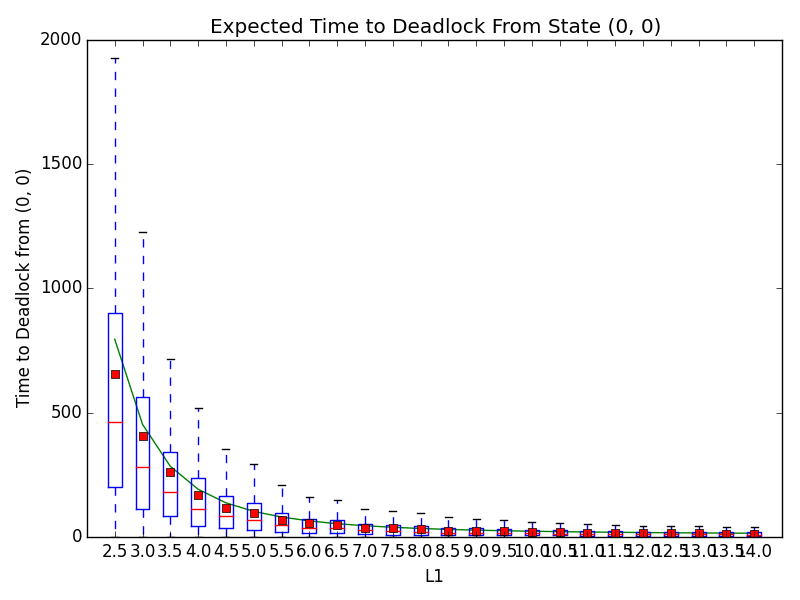
\includegraphics[width=\textwidth]{images/varyL1}
  \caption{Varying $\Lambda_1$}
  \label{fig:timestodeadlock2_L1}
\end{subfigure}
\begin{subfigure}[b]{0.5\textwidth}
  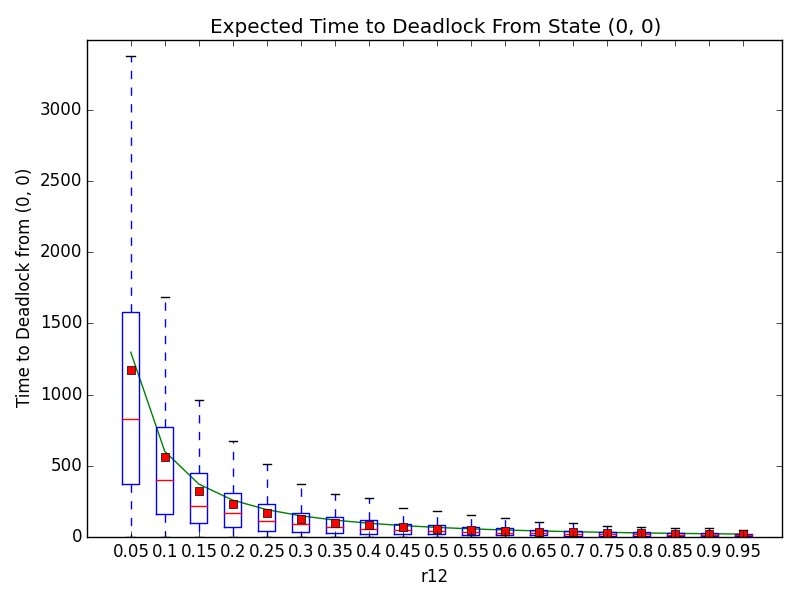
\includegraphics[width=\textwidth]{images/varyr12}
  \caption{Varying $r_{12}$}
  \label{fig:timestodeadlock2_r12}
\end{subfigure}
\begin{subfigure}[b]{0.5\textwidth}
  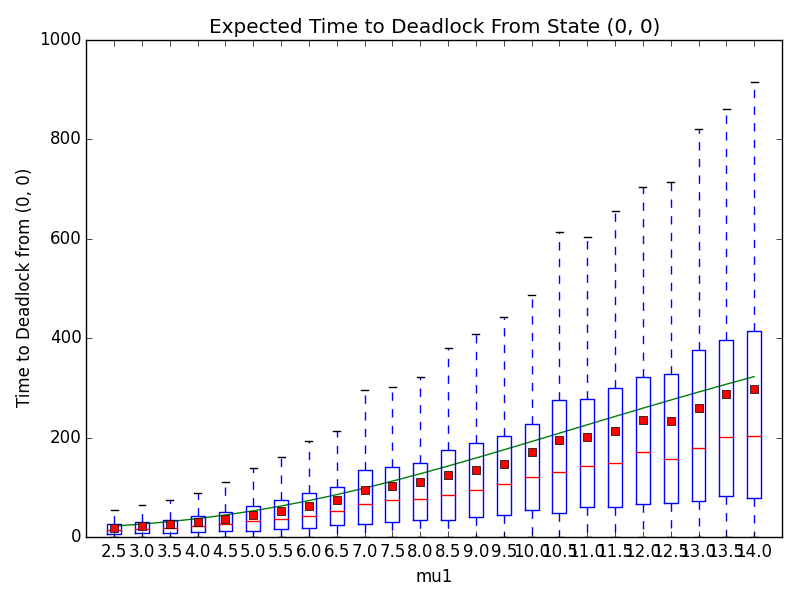
\includegraphics[width=\textwidth]{images/varymu1}
  \caption{Varying $\mu_1$}
  \label{fig:timestodeadlock2_mu1}
\end{subfigure}
\begin{subfigure}[b]{0.5\textwidth}
  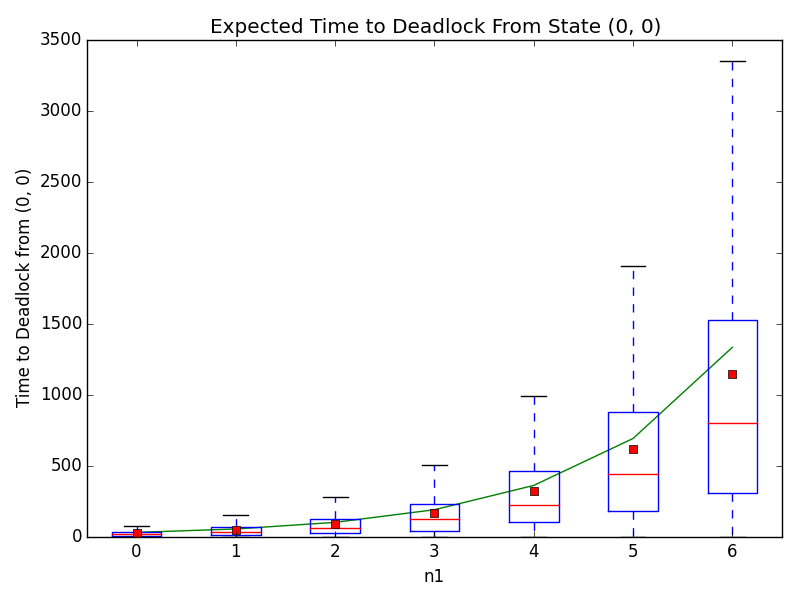
\includegraphics[width=\textwidth]{images/varyn1}
  \caption{Varying $n_1$}
  \label{fig:timestodeadlock2_n1}
\end{subfigure}
\caption{Analytical \& Simulation Results of Times to Deadlock (1000 iterations)}
\label{fig:timestodeadlock2}
\end{figure}


\subsection{Resolving Deadlock}
Once the system falls into a deadlocked state for the first time, that is the first transient deadlocked state since the last resolution, the simulated needs to automatically resolve the deadlock and allow services to resume again.
This is not necassarily as simple as moving a blocked customer to his next node, as we need to conserve the numbers of customers at each service station.
Closer inspection of the state digraph is required in order to find a way to resolve deadlock whilst conserving this property.

At deadlock, the service stations can be classified into the following three mutually exclusive categories:
\begin{itemize}
    \item Nodes that are not deadlocked: These are nodes that do not contain any blocked individuals.
    \item Causation nodes, nodes causing deadlock: These are nodes where every server is occupied by a blocked individual, and there is at least one blocked individual waiting to enter that node who is directly or indirectly being blocked by an individual in this node.
    \item Affected nodes, nodes affected by deadlock: These are nodes containing at least one blocked individual who is directly or indirectly being blocked by an individual at a node that is causing deadlock, but is not classified as causing deadlock itself.
\end{itemize}

At the first instance of deadlock, there will only be one knot in $D(t)$.
Let us denote the knot as $K$.
The vertices of $K$ correspond to servers.
As there is no sink node, all vertices of $K$ have an out-edge, and so all vertices in $K$ contain a blocked individual.
Therefore, there are no vertices in $K$ belonging to nodes that are not deadlocked.
All vertices of $K$ correspond to servers of causation nodes, and a causation node has all its servers belonging to $K$.
An affected node has servers belonging to the same weakly connected component as $K$, but does ot have servers in $K$.

When choosing which customer to move in order to resolve deadlock, we must be careful to conserve the number of customers at each service station.
Causation nodes have full queues, and a customer may only be moved into a full queue if this causes another customer to simultaneously move from this node.
Another complication arises due to the blocking mechanism used, in which those customers who have been blocked longer must be moved first.
This property may have to be broken in order to ensure the conservation property is not.
Assume that we have weighted the edges of the digraph with the time that they were created. % If this works then I'll include this in the write up of how state digraph is formed

The following algorithm is proposed in order to resolve deadlock:

\begin{algorithm}[H]
    \DontPrintSemicolon
    Find the knot $K$ in $D(t)$\;
    Find the cycle $C \in K$ whose average edge weight is minimum\;
    Start at $V_0$\;
    \For{$V_i$ in $C$}{
    Move the individual who is waiting to get to $V_{i+1}$\;}
    Redraw $D(t)$\;
\end{algorithm}



\bibliographystyle{plain}
\bibliography{references}

\end{document}
